\chapter{Experimental Methods}
\label{Chap:Methods}

The following Chapter introduces a selection of experimental methods and techniques relevant in the context of the laser wakefield acceleration (LWFA) experiments. The three main ingredients of an LWFA experiment will be covered: a high-intensity laser, gas targetry and diagnostics for particles and secondary radiation.

%The chapter starts by introducing high-intensity lasers and a brief outline of chirped-pulse amplification (CPA), the main tool to drive and probe the plasma wave, and how to diagnose it in experiment.
The Chapter starts by introducing the Gemini laser system, the dual-beam high-intensity laser used to conduct the experiments in this work, and diagnostics to characterise the laser.

It then continues with a section on gas targets used in LWFA experiments, focusing on targetry that is specifically relevant to the experiments discussed later.

Finally, the techniques used to diagnose the plasma, the interaction of the laser with the plasma as well as particles and radiation generated in the process are introduced.
\EliasComm{Change intro, maybe more focus on radiation diagnostics.}
A more comprehensive review of diagnostics is provided in \cite{Downer2018_DiagnosticReview}.

\section{The Astra-Gemini laser and Target Area 3}

All of the experimental results presented in this work were acquired at Target Area 3 (TA3) using the Astra-Gemini laser \cite{Hooker2006_Gemini,Hooker2008_Gemini} of the Central Laser Facility (CLF) at the Rutherford-Appleton Laboratory (RAL), UK.

The titanium-sapphire-doped (Ti:Sa) Gemini laser with central wavelength $800\,\mathrm{nm}$ provides two beams every 20 seconds at a compressed pulse duration of down to $40\,\mathrm{fs}$ and up to $10\,\mathrm{J}$ energy on each arm. The collimated beams that enter the target chamber have a diameter of $\sim 150\,\mathrm{mm}$ with a flat-top intensity profile and are focused down either with a spherical mirror or off-axis parabolas (OAPs). Adaptive optics (AOs) are deployed on both laser arms in conjunction with wavefront sensors to remove aberrations and flatten the wavefront.

In the context of the LWFA experiments discussed later typically two types of geometries are of relevance at Gemini:

\iffalse
\begin{figure}
\centering
\includegraphics[width=.75\columnwidth]{chamber1.jpg}
\caption{Photo of the Gemini TA3 vacuum chamber. PhD student to scale.}
\end{figure}
\fi

First, a long-focal-length geometry using either an $f/40$ spherical mirror or an OAP with $f = 6\,\mathrm{m}$ to provide an intense laser pulse $a_0 > 1$ with a long Rayleigh length, $z_R$, to efficiently drive LWFA over long distances. Due to the long focal length and the limited size of the Target Area the beam has to be reflected or `folded' at least once during the focusing process, in recent setups about halfway between optic and focal plane. Unfortunately, this means that the usable maximum energy in this laser arm is limited by the damage threshold of these `folding' mirrors or in other words the fluence the mirrors can sustain. The threshold at which damage occurs depends on several factors, including the beam quality and beam size, the quality of the mirror coating and cleanliness of the chamber.

The second geometry is the short-focal-length scatterer which is typically an $f/2$ OAP with focal length $f = 300\,\mathrm{mm}$ which is also available with a central fitted hole for the case of head-on counter-propagating geometries. 

In addition to its full-power capabilities, a continuous-wave (CW) mode for alignment and a low power pulsed mode at 10 Hz repetition rate are available as well.
\EliasComm{Review}

\section{Laser Diagnostics}

\iffalse


Since the experimental realisation of the laser \cite{Maiman1960} it has taken an indispensable role in a wide range of fields covering communication, construction, navigation, medicine, pharmaceuticals, machining, defense, numerous applications in science and innovation and more. 

The advent of chirped pulse amplification (CPA) \cite{Strickland1985} enabled the generation of short and intense laser pulses paving the way for precision machining, medical tools used in cornea and heart surgeries, but also multi-photon science, non-linear optics and in the context of this work the wakefield acceleration in the so-called 'bubble' or 'blowout' regime, generating a directed relativistic quasi-monoenergetic electrons from a laser-plasma interaction.

In physics, the push towards higher intensities and shorter pulse durations allows us to understand matter more and more and how it interacts with light on a fundamental level, opening up a field of interesting new phenomena and applications to investigate \cite{DiPiazza2012}.
\EliasComm{What was the role of the laser in physics?}
\vspace{\baselineskip}

%At the beginnings of the experimental work in the field of wakefield acceleration, high intensity short pulse lasers as the ones that achieved the breakthrough for LWFA in 2004 (quasi-monoenergetic electrons in the MeV regime \cite{Mangles2004,Faure2004,Geddes2004}) were not available.
%Restricted by the breakdown threshold of the amplification crystals the pulse duration and intensity were limited. In order to still drive wakes creative acceleration schemes were developed to compensate the lack of more powerful short-pulse lasers. Examples are for instance the beat wave plasma accelerator \cite{Tajima1979} or the self-modulated plasma accelerator.

With the advent of short pulse terrawatt systems after the invention of chirped pulse amplification (CPA) \cite{Strickland1985}, wakefield acceleration achieved a breakthrough reaching the highly non-linear regime, referred to as the `bubble' regime, and the production of quasi-monoenergetic electrons in the MeV regime \cite{Mangles2004_MONO,Faure2004_MONO,Geddes2004_MONO}.
CPA opened up the relativistic regime at intensities of around $10^{17}-10^{18}\,\mathrm{W}\,\mathrm{cm}^{-2}$, where electrons accelerate to relativistic velocities within a single laser period leading to interesting effects like relativistic self-focusing which is also used to achieve longer guiding in LWFA. Even intensities of $10^{21} \,\mathrm{W}\,\mathrm{cm}^{-2}$ are within reach where QED corrections become relevant and phenomena like radiation reaction (classical and quantum), multi-photon Compton scattering or even the quantum vacuum itself can be investigated. The current record exceeds a peak intensity of $10^{22}\,\mathrm{W}\,\mathrm{cm}^{-2}$ and laser systems pushing this even further by orders of magnitude are being planned or built already, as for instance the facilities of the Extreme Light Infrastructure (ELI) REFERENCE HERE or the proposed upgrade of the Vulcan laser at the Central Laser Facility in the UK (REF).
\EliasComm{Some doubling in this paragraph}
\vspace{\baselineskip}


%\subsection{Chirped-pulse amplification (CPA)}

In laser amplification a laser pulse passes once (single pass) or multiple times (multipass) through an amplifier medium, called the laser gain medium, and is amplified in the process. To generate ultrashort pulses a large bandwith gain medium is required in order to amplify continuously over a large frequency domain. A popular choice are lasers based on titanium-doped sapphire (Ti:Sa) as gain medium due to their large bandwidth and tunability. At short pulse durations and high intensities non-linear effects such as relativistic self-guiding start to occur, leading to a local increase of the field strength. At very high field strengths the gain medium starts to ionize and in turn to take damage: amplification of these short pulse lasers is limited by this breakdown. Further amplification can then only be achieved if the beam is expanded for which then a larger gain medium becomes necessary. This limitation was overcome or at least pushed further by the invention of chirped-pulse amplification (CPA) \cite{Strickland1985} based on a technique employed in radar technology.
\vspace{\baselineskip}

CPA takes advantage of the fact that short laser pulses are not monochromatic but a spectrum. This is a necessary property for the pulse to have a short duration, an evident feature when considering the Fourier transformation.

CPA exploits this fact and stretches the pulse in time using sets of refraction gratings: depending on the frequency of the light it will be refracted differently, extending or shortening the path relative to other frequencies. A pair or a couple of grating pairs can in this way stretch the pulse with a dependence on wavelength: the pulse is `chirped'. In the pioneering work of Strickland and Mourou a long glass fibre was used to stretch the pulse coupled to a grating to compress it again \cite{Strickland1985}. The energy density of the stretched pulse is now much lower than before and the pulse in total can be amplified to much higher intensities without damaging or saturating the gain medium. In the next step, a set of gratings reverse the process and compress the pulse, achieving a high intensity but also an ultrashort pulse duration that is ideal for LWFA.
\vspace{\baselineskip}


However, even with CPA the amplification achievable is finite as it is not useful to stretch the laser pulse arbitrarily much to lower the energy density and an ordinary gain medium as amplifier will reach its limits again as soon as the stretched pulse reaches the ionisation threshold. In addition, the gratings have to withstand these high intensities when recombining the stretched pulse and hence have to have a high damage threshold. An improved chirped-pulse amplification scheme to push this boundary even further is the so called optical parameter chirped-pulse amplification (OPCPA) scheme. The normal amplifier crystal is substituted by a non-linear medium. The laser pulse deposits only a fraction of energy of the amount in ordinary laser gain media as it works via a parametric process, which allows to pump this medium with even higher powers.

Another alternative is combining several separately amplified laser pulses either incoherently or coherently (add references REF).


\begin{figure}
\centering
\includegraphics[width=0.8\columnwidth]{Chirped_pulse_amplification.png}
\caption{Schematic layout of a CPA system\protect\footnotemark. The initial short pulse is sent through a grating which disperses the spectrum of the pulse and stretches it, resulting in a longer pulse with a monotonic frequency shift throughout: the pulse is chirped. The pulse with lower power is amplified and re-compressed in another set of gratings to a short and high-power pulse.}
\end{figure}


\footnotetext{Graphic taken from Wikipedia: \url{https://en.wikipedia.org/wiki/Chirped\_pulse\_amplification}}

\fi



\subsection{Laser Energy Measurement}

At Gemini, the laser energies are measured on every shot by collecting the transmitted light through the back of a highly-reflective dielectric mirror in the laser area and imaging it onto a CCD camera chip. The integrated number of counts is calibrated using a Gentec\addref laser energy meter and the filtering is adjusted for different power modes.

A Gentec is also used to measure the reflectivity of the compressor gratings, typically between 60 ad 70 percent, and the energy reaching the interaction point.

\EliasComm{Calorimeter?}

\subsection{Laser Pulse Duration Measurement}

At Gemini, frequency-resolved optical gating (FROG) \cite{FROG} is used to measure the pulse duration of the laser and characterise its temporal intensity profile.
A FROG trace can be taken on every shot by using the through high-reflective dielectric mirrors transmitted beam in the laser area.

The FROG is a diagnostic to measure the intensity and spectral phase of ultrashort laser pulses as present at Gemini ($\sim 40\,\mathrm{fs}$). The setup is similar to an autocorrelator and is optically gated by combining two beams in a non-linear medium. Typically a second-harmonic-generation (SHG) crystal is the non-linear medium of choice. The produced second-harmonic (SH) radiation is then spectrally resolved (hence frequency-resolved) and provides information about the spectral phase.

More details can be found in \cite{FROG} or, for instance, also in Matthew Streeter's PhD thesis \cite{StreeterThesis}.
%\vspace{\baselineskip}


%A dazzler (REF) can be used to fine-tune the pulse profile.

%Other diagnostics that can be used to measure the pulse duration are the SPIDER (REF) or an autocorrelator (REF), but they are not single-shot diagnostics and require scans.

\subsection{Focal Spot Characterisation}

In LWFA a short-pulse laser is focused down to reach high enough intensities to drive a wake, but has to guide itself over a long range at the same time. In parts of this work a second laser is used as scatterer for inverse Compton scattering or as an X-ray heater.

For each of these applications it is important to optimise and characterise the size and spatial energy distribution of the focal spot. Combining this with a measurement of the temporal pulse shape, for instance using a FROG, then provides an intensity map of the laser pulse at focus.
\vspace{\baselineskip}

In this work a CCD camera (AVT Manta G-033B) is coupled to a near infrared (NIR) infinity-corrected apochromatic long-working-distance microscope objective (depending on the application Mitotoyo X10 or X20 magnification) to image the spot at its focal plane. 
A thin metal wire of $10's-100 \,\mathrm{\mu m}$ width is used to help defining a focal plane.
\vspace{\baselineskip}

Due to the high intensity Gemini can reach the beam alignment and also the characterisation of the focal spot are performed with the CW mode or the attenuated low-power pulsed beam. Assuming the focal plane and general character of the spot remains the same, the energy of the actual focal spot on shot is then scaled from the low power image.

A real direct measurement of the actual focus at typical intensities used in wakefield experiments is very challenging. Recent attempts involved the full 3D characterisation of the wavefront of the collimated laser beam by applying an asymmetric Mach-Zehnder interferometer and scanning the entire beam profile over hundreds of shots \cite{TERMITES} or using a gas jet ionisation (REF HERE). 

\begin{equation}
a_0 \approx 0.85 \lambda [\mu m] \sqrt{I [10^{18} cm^{-2}]}
\end{equation}


\subsubsection{Image Processing}

In addition to a spatial calibration, the images for a focal spot analysis require some background removal: 
A series of images without any laser are taken (dark field) and averaged over to be then subtracted from the actual focal spot image. 
Then a median filter can be used to account for individual hot pixels on the camera.

The remaining signal should be mainly the laser spot and the highest pixel values are at the centre of the focal spot.
Taking the maximum pixel value and fitting an ellipse to area reaching half of this value, the \textsc{fwhm} size of the spot is estimated.
The area of the focal spot, ignoring smaller deviations from an ellipse, is then $A = \pi a b$, where $a$ and $b$ are the two axes.
Comparing the pixel counts within the \textsc{fwhm} contour against the pixel counts in the total beam, one can then quantify the fraction of energy contained in the \textsc{fwhm} the beam. A high fraction is important as the wings of the beam decreases the peak intensity and will not be guided in the wakefield accelerator, is hence lost.

\subsubsection{Spatial calibration}

As the exact size of the focal spot is important, the focal spot camera has to be spatially calibrated. Carefully measuring the distances between the components of the optical system and knowing about their properties might not be accurate enough. Alternatively, the camera can image an object of well-defined spatial extent. A typically tool are USAF targets, for instance provided by Thorlabs, available in transmissive or negative, with a range of line sets of different dimensions. Knowing the pixel size of the camera one can then relate the width of the lines to a conversion factor from pixels to microns, in this case. Another approach is placing a grid of known dimensions into the collimated laser beam and deduce the spatial dimensions by measuring the separation of the diffracting multiple copies of the focal spot following:
\begin{equation}
\sin \theta = \frac{m \lambda}{d} \rightarrow x_m = m f \tan \theta \rightarrow x \approx \frac{f \lambda}{d}
\end{equation}

\iffalse
\begin{figure}
\centering
\includegraphics[width=0.5\columnwidth]{FocalSpot_USAF_example.png}
\caption{Example USAF.}
\end{figure}
\fi


\subsubsection{Intensity Estimate}

Knowing about the total energy in the beam and combining this with a measurement of the pulse shape (e.g. using a FROG), the number of pixel counts in the spot can be related to an intensity in the beam.
The focal spot in figure XXX for instance has a size of XXXXXXX. The FROG analysis indicates a peak power of XXX TW. Combined this gives a peak $a_0 = 2$. 

Ideally, a series of several focal spots, even hundreds, are taken to incorporate fluctuations in the shape of the spot but also to characterise the typical spatial fluctuations over time.

\subsection{Wavefront Sensor and Adaptive Optics}

Real laser beams tend to have a series of imperfections attributed to them due to the gain medium, diffraction, dirt or damage on optics, misalignments, beam transport and so on.
Too many aberrations or distortions in the beam prevent it from focusing down to a close-to-idea diffraction-limited spot and result in energy being distributed in wings instead of merging to a small spot. As a consequence the reachable peak intensity is lower and a large fraction of energy is not efficiently used in the process. 
\vspace{\baselineskip}

In addition to ensuring that the beam propagation and source is as close to ideal as possible, one can use a wavefront sensor to characterise the wavefront of the beam. In conjunction with a deformable mirror or an adaptive optic (AO) a software can derive a map relating changes in the mirror to changes in the wavefront. Using this map or `interaction matrix' the mirror can be applied to flatten the wavefront iteratively correcting for wavefront errors which makes consequent modelling easier, matching to simulations, and enables reaching a diffraction limited focus at higher intensities.
On the other hand, this also gives control to add aberrations and tailor the wavefront to specific applications that might benefit from this, e.g. astigmatism for on-shot reference measurements in radiation reaction studies \cite{Baird2019_RR}, wavefront tilt to enhance the emission of betatron radiation \cite{Mangles2009_BETATRON}.
\vspace{\baselineskip}

In this work a Shack-Hartmann sensor (HASO DETAILS REF) was used. This type of wavefront sensor consists of an array of microlenses.
A HASO observes the temporally integrated wavefront profile of the laser pulse. Spatio-temporal couplings are not visible and have to be diagnosed differently, for instance by characterising the behaviour of the beam near its focus or by measuring the focus separately for different temporal slices (using narrow interference filters).

One adaptive optic was an ILAO (mechanical motors, large stroke) made by the French company XXX, the other one is a piezo-activated AO made by Chris Hooker at RAL.


\section{Dual-Beam Timing Diagnostics}

In experiments involving two or more pulsed laser beams, for instance pump-probe or colliding-pulse experiments, the beams require spatial and temporal synchronisation down to the $ps$ or even $fs$ level.
Depending on the accuracy required different techniques can help measure the difference in timing, as well as correct and monitor the synchronisation over extended periods of time.

Photodiodes, spatial and spectral interferometry are introduced. This is not an exhaustive list and other methods, e.g. cross-correlator, are not introduced as they were not used explicitly in the experiments presented.
\vspace{\baselineskip}

At Gemini both laser beams originate from the same source (oscillator) and are hence `intrinsically' synchronised, which means that they are emitted/triggered at the same time, underlie the same jitter but do not shift relative to each other at the point of emission. However, this does not mean that both beams are automatically synchronised at the point of interaction, since the arms take different pathways through the amplification and compression stage, and then finally follow different beam lines within the target chamber. The longer their separate paths the larger the potential impact of, for instance, vibrations and thermal effects can be. Incredibly small changes can cumulatively make a significant impact on the $\mathrm{fs}$-scale synchronisation required in some of the challenging experiments attempted at Gemini.
\vspace{\baselineskip}

`Timing' two beams means in this case that the relative path lengths are adjusted to compensate for the measured difference in the time of arrival at the interaction point. At Gemini larger distances (few nanoseconds or metres in distance) require moving optics physically to extend the beam path, smaller distances are finely adjusted by using a linear translation stage that adds or removes path length in double-pass at few femtosecond (micrometre) precision. This stage is on the `split-and-delay' (SAD) table in the LA3 laser area. The linear stage is a Newport XXX REF.

\subsection{Diode Timing}

Photodiodes are a useful and easy-to-use tool to measure the temporal separation of light signals on a nano- to picosecond scale.
Rise and fall times for fast diodes are few tens of picoseconds placing the peak of the distribution within $\sim10\,\mathrm{ps}$ using an appropriate oscilloscope. 

Both laser pulses have to be overlapped at the designated point in space and the signals combined onto the diode. Alternatively, an object at the crossing point can be used to scatter both beams to send a more diffuse signal to the diode. This is a suitable method if the extent of the scattering object is negligible on the order of the accuracy of the method.
\vspace{\baselineskip}

\begin{figure}
\centering
\includegraphics[width=0.5\columnwidth]{PhotoDiode_BW.jpg}
\caption{Photodiode.}
\end{figure}

In the experiments at the Gemini laser the fast EOT-4000 GaAs photodetector with a rise/fall time of $< 30\,\mathrm{ps}$\footnote{Details can be found on the Electro-Optics website. www.eotech.com} was used in conjunction with a Lecroy WaveMaster 813Zi-B oscilloscope ($>13\,\mathrm{GHz}$)\footnote{More details on Lecroy XX WEBSITE XX}. This limits the resolution of the signal to about XXX PS. The accuracy of the difference measurement is per measurement is a few picoseconds. If several measurements at different separations (using a delay stage to delay one laser arm) are taken the error can be reduced to an accuracy of XXX PS.
\vspace{\baselineskip}

The detectors were only used at air and are not compatible for vacuum use.
\EliasComm{This is also as we need short and thin cables to make use of the fast oscilloscope and this would not work with a feedthrough.}

\subsection{Spatial Interferometry}

\subsubsection{General}
Diode timing is limited by the typical rise and fall times and the access to a fast oscilloscope.
A different method that is more coupled to the pulse duration of the laser beams is spatial interferometry. 
If both laser pulses have the same polarisation and are overlapped in space and time, both beams can interfere. 
Due to the large bandwidth of the Ti:Sa laser pulses used in this context the coherence length is very short and interference will only take place over the combined pulse duration, i.e. a potentially small time window. This is why this method is a useful technique to achieve precise timing after using a diagnostic with a wider time window (but less precision) like the photodiodes introduced in the previous section.


\begin{figure}
\centering
\includegraphics[width=.75\columnwidth]{RR19_TCC.png}
\includegraphics[height=0.4\columnwidth]{Fringes_spatial_F2F20.png}\includegraphics[trim={14cm 0 0 0}, clip,height=0.4\columnwidth]{Fringes_spatial_exp.png}
\caption{RR19 TCC with spatial interferometry setup. Fringe simulation and experimental results for f/40 and f/2.}
\end{figure}


\EliasComm{Add here an example for Gaussian beams and the equation for interference based on this.}

\begin{equation}
\boxed{I \sim |1+\cos(ky \sin\theta - \omega \Delta \tau + \phi )|}
\end{equation}

As we see the interference fringes rely on a phase difference between the two laser pulses. The main contributor for two timed spectrally identical laser pulses are a relative angle or different radii of curvature.
The experiments presented combine a short focal length optics with a longer focal length beam line and hence perfect alignment can be aspired to as the interference pattern will be clearly visible due to the stark difference of the radii of curvature of, for instance, and f/40 and f/2 at the relevant point.

\subsubsection{Experimental Implementation}

In the experiments described in Chapters RR15 XX and RR19linICS XX spatial interferometry was used. 
Both beams were reaching the interaction point at 180 degrees from each other. One f/2, the other f/40. A 90-degree knife-edge prism with reflective surface was driven in at the desired interaction point and used to deflect both beams collinearly onto the CCD chip of a camera, in this case equipped with a x10 long-working-distance microscope objective.

The contrast of the interference pattern was adjusted by equalising the relative brightness of the beams with a combination of adjusting the distance of the camera to the prism edge taking advantage of the different focal lengths and by adjusting the rotation angle of the polariser as the beams are cross-polarised.

These measurements were done using the pulsed low power beam at Gemini.

\subsection{Spectral Interferometry}

In spectral interferometry two identically chirped pulses are spectrally dispersed using a grating and the individual spectral components overlap and interfere. Due to the dispersion the coherence length is greatly increased as $L \sim \Delta \lambda^{-1}$ and the interference pattern is visible over a much larger time window than for spatial interferometry.

Visible over hundreds of femtoseconds and hence over a much larger time duration than for spatial interferometry, tens to hundred picoseconds.

A grating is required coupled to a detector, e.g. CCD camera.
This could simply be a spectrometer with suitable grating \cite{Corvan2016_TIMING}.

\begin{align*}
S(\omega) &= |FT[E_N (t) + E_S (t +\Delta \tau)]|^2\\
&= |\tilde{E}_N(\omega)|^2 + |\tilde{E}_S(\omega)|^2 + 2 |\tilde{E}_N(\omega) \tilde{E}_S(\omega)|\cos(\omega \Delta \tau + \phi_N(\omega) - \phi_S(\omega))
\end{align*}

The fringes now depend on the temporal separation of the beams in the dispersive direction.
This means an absolute number for the temporal separation can be acquired instead of a single binary signal for the overlap. 
This diagnostic is also able to track changes in absolute terms and suitable to track changes in timing over extended time periods.

\begin{figure}
\centering
\includegraphics[width=0.8\columnwidth]{Fringes_specTA3_exp.jpg}
\includegraphics[width=0.8\columnwidth]{Fringes_specLA3_exp.jpg}
\caption{Fringes from TA3 and LA3.}
\end{figure}


\subsubsection{Experimental Implementation}

Off-shot diagnostic combining the beams onto a grating and a CCD chip.

Using leakage beams at two locations in Gemini. Then combine into imaging spectrometer.
One built by Nicolas Bourgeois, the other one by Matt Streeter based on Rob Shalloo (RAL Report).

\EliasComm{Add pictures from the Staging19 campaign.}

\subsection{Considerations for Timing Beams}

Synchronising two laser beams to each other or a laser with an electron beam in an experiment down to the femtosecond level comes with many challenges and considerations.


Light moves slower through media than through vacuum. The group velocity is reduced to $v_g \approx c(1-1/2 (\omega_p/\omega)^2)$ or $v_g =c/\eta$.
In experiment this means that introducing or removing media asymmetrically from beam paths will change the relative time of arrival.

Typical examples at Gemini are moving from air to vacuum (pumping down the vacuum chamber), removing or adding gate valves, or attenuating beams using glass slides, when switching power modes.

\subsubsection{Shifts from Air to Vacuum}

The refractive index, $\eta_0$, of vacuum is $\eta_0 = 1$.
The refractive index of air at standard temperature and pressure for 800 nm is $\eta_{air} = 1.00027$ (REF NIST)\footnote{add REF here.}
\begin{align}
\Delta t &= \frac{d}{c} \left( \eta_{air} - \eta_{0}\right),\nonumber\\
\Delta t  &\approx 0.9\,\mathrm{ps} \times \frac{d}{1\,\mathrm{m}},
\end{align}

which means every metre of path length that is being shifted from air to vacuum will add $0.9\,\mathrm{ps}$ of time delay.
If the beam path of the two beams are asymmetric, the difference in beam path times this change in time from air to vacuum will lead to a change in timing as well.

At Gemini the driver beam typically covers a path of over 10 m distance as it includes long-focal-distance optics with $f = 6\,\mathrm{m}$ whilst the scatterer beam only covers about half of the distance. A difference in $5\,\mathrm{m}$, for instance, would then mean that the driver beam arrives at the interaction point $4.5\,\mathrm{ps}$ after the scatterer.

\subsubsection{Gate valves}

Another step in the pump-down process at Gemini is opening the gate valves that separate the target chamber, which is often at air or lower quality vacuum, from the relatively permanent and high quality vacuum of the laser compressors (two separate compressors).
Once the vacuum in the target chamber reaches a sufficient quality and the turbo pumps are engaged, the gate valves are opened.
The gate valves at Gemini are made out of sapphire glass but are of different thickness on each arm \cite{GEMINI_GATEVALVES}. The difference in thickness is around $60 \pm 3\,\mathrm{\mu m}$.

The refractive index is 1.75 and 1.76 in ordinary and extraordinary axis at 800 nm. This means removing the gate valves will shift the relative time of arrival again by $150\,\mathrm{fs}$.

\subsubsection{Attenuation of beams}

The previous two examples can be cross-checked by repeating some of the timing procedures, for instance using spatial interferometry after the pump-down, add the correction factors and optimise the interference pattern again.

In some cases, however, material might be inserted asymmetrically to attenuate the beams. At Gemini glass slides are available to attenuate beams by a factor $\sim 100$ and are used in conjunction with polarisers and waveplates to improve the contrast of the interference pattern.
The attenuators are $2\,\mathrm{mm}$ thick fused silica glass slides at 45 degrees with refractive index $\eta = 1.4533$\footnote{NIST ref or so} REF, introducing a $4.24\,\mathrm{ps}$ delay per attenuator (up to 2 per beam). In this setup the attenuators are identical and if an equal number are used per beam no measurable change in relative time of arrival is witnessed. An asymmetric number requires adjustments and in general if materials are inserted, it should be checked whether they might influence the time of arrival.
\vspace{\baselineskip}

Recently, the attenuators at Gemini have been matched with `compensator plates' that will be in the beam path when the attenuators are removed. The compensator plates and the attenuators are matched, such that introducing an attenuator should not change the delay at all and asymmetric attenuation also would not change the relative delay. The accuracy of this setup, however, also has to be investigated and quantified.

\subsubsection{Laser-Laser to Beam-Laser Timing}

So far the considerations and methods have been aimed at ensuring the temporal overlap of two laser pulses, taking into account changes introduced by pump-down procedures or attenuation. Finally, we want to highlight what to consider when aiming to synchronise a laser pulse to an electron bunch accelerated through LWFA, relative to a laser-laser synchronisation.
\vspace{\baselineskip}

In LWFA, the driver beam propagates through a plasma and is hence slower relative to the in vacuum-timing procedure: it will arrive later at the interaction point than measured previously in vacuum.

The electrons are injected after a certain distance of propagation. After injection they quickly reach a velocity close to the speed of light, from when the electrons and the second laser pulse travel at approximately the same velocity.

For the relative offset of the driver pulse and the electron bunch we can estimate that the bunch trails in the Nth bubble behind the laser pulse between N/2 to N plasma wavelengths, the accelerating to zero phase region of the bubble. If the electrons are close to dephasing and in the first bubble, the laser-electron offset is 1/2 $\lambda_p$.
\vspace{\baselineskip}

This shows that knowing the point of injection becomes important. Alternatively, calculate the distance the laser pulse propagated in plasma and take this as total delay (as the electrons are moving just as fast as the laser in vacuum from thereon forwards). For this purpose measuring injection radiation or forcing radiation at a designated point (shock injection) becomes very useful.

However, this assumes that the electron bunch does not have a spatio-temporal extent which is typical for LWFA beams with long tails and potentially energy-time chirp. Short, localised injections will lead to low energy spread but also short bunches that will localise the beam further. This is also a property shock injection can facilitate.
\vspace{\baselineskip}

Another example of electron-laser timing, but in the context of PWFA, is the plasma afterglow \cite{Scherkl2019_PLASMAAFTERGLOW}.
At FACET-I a conventional accelerator provides the electron bunch, so the timing can not be performed in the same way.
By overlapping the electric field of the electron bunch and a laser in a gas jet, one can infer from the ionisation rates when both were overlapped in time and space. This has been used for \cite{Deng2019_TROJAN}

\subsubsection{Drifts in Timing}

In addition to the examples mentioned so far, when trying to synchronise two laser pulses or a laser and an LWFA electron beam, one also has to consider the stability of the synchronisation. At Gemini, the laser pulses cover typically several 10's of metres distance in several rooms before finally being directed into the target area. Minor changes in the environment (humidity, temperature) can lead to expansion or contraction of optical tables and components leading to a drift of the alignment and the relative timing over a period of time. See \cite{Shalloo_GEMINIDRIFT} where the relative timing was measured and monitored over an extended period of time, highlighting the importance of a stable environment in the laser area and the target area.

Whilst it is of utmost importance to minimise these effects by investing in climate-controlled laboratories, it also shows that at the femtosecond level of precision the actual on-shot measurement of the timing and alignment becomes important to gain real control over interactions.

\section{Gas Targets}

In laser-wakefield acceleration (LWFA) the laser pulse propagates through the plasma and sets up a density modulation. To permit this propagation the density of the medium has to be below the critical density, $n_c = m_e \epsilon_0 \omega^2/e^2$. A medium with electron density $n_e < n_c$ is referred to as `underdense'. At $\lambda = 800\,\mathrm{nm}$ these are typically gaseous targets. `Overdense', i.e. targets with a density higher as the critical density, are mostly solid or liquid targets in the context of Ti:Sa lasers. They are preferrably used for ion acceleration schemes (e.g. (Target Normal) Sheath Acceleration (TNSA) \cite{Wilks2001_IONACC,Maksimchuk2000_IONACC} or to generate X-rays (REF). In LWFA experiments, however, densities well below $n_c$ are required. 
\vspace{\baselineskip}

Gas and liquid targets offer the advantage of being used in high-repetition experiments as they can be destroyed and replenished in a short amount of time without significant re-alignment and debris production. The limiting factors for the repetition rate are the performance of the vacuum system, the time it takes the gas flow to reach equilibrium, the durability of nozzles/casings etc. and the repetition rate of the laser system in use. Facilities like FLASHForward that have in principle the capabilities and the ambition to operate at MHz repetition rate (REF) even have to consider ion and plasma dynamics and scintillation times for detectors.
\vspace{\baselineskip}

Examples of gas targets that are routinely used for wakefield experiments are gas jets \cite{Semushin2001_GASJETS}, gas cells or capillaries \cite{Leemans2006_GEV,Leemans2014_GEV,Nakamura2007_GEVGUIDED,Desforges2014_CAPILLARY} (REF SIMON HOOKERS GROUP? JENS GROUP?) and capillary targets with a pre-ionised plasma (using an electric discharge) \cite{Spence2001_WAVEGUIDE}. In some cases several targets of the same or different type or combined and staged together to achieve more favourable results.
However, even within those types of targetry a large variety exists, with each target being tailored to a different application and purpose. 

The target size, i.e. the distance the laser pulse has to propagate through the medium, has to be matched with the laser in use, considering depletion and dephasing lengths to optimise the particle and radiation output, and to use the energy of the laser pulse to its fullest.


As listing and explaining all those different targets would be a hopeless task, the focus will be on examples of gas jet and cell specimen relevant to the work presented within the course of this thesis.

\subsection{Gas Jets}

The flow of gas produced when forcing it with high backing pressure through a small orifice at the bottom of a diverging cone is in the context of this work related to as gas jet.
If the measurements of the cone are chosen correctly at a high enough backing pressure, the flow detaches and becomes supersonic \cite{Semushin2001_GASJETS}
Supersonic gas jets are able to produce relatively smooth flat-top density profiles with short density ramps on both sides, suitable for LWFA.

The density of the gas jet is controlled by varying the backing pressure of the gas line, where higher pressure results in higher densities. When comparing nozzles of the same type in different sizes, larger nozzles require higher backing pressures to reach the same densities as smaller nozzles. For supersonic flat-top profiles the density slowly decreases above the nozzle. The actual density profile and gas flow depends on the specific design and manufacturing.
\vspace{\baselineskip}

\iffalse
The expanding gas cools down and in some cases can lead to the formation of clusters held together by the Van-der-Waals force between the atoms or molecules \cite{Hagena1972}. Clusters are being investigated as gas targets with potentially higher charge or beam stability as in self-injection (REF). Suprasonic flows on the other hand might be useful for other applications including the production of betatron radiation (REF). 
\vspace{\baselineskip}
\fi

Gas jets provide a relatively easy target, diverse in shape and comparatively straightforward to align. The open geometry also allows optical probing from a large solid angle. However, experimental results are less stable (shot-to-shot reproducibility) and inferior in terms of maximum energy \cite{Leemans2014_GEV} and stability \cite{Desforges2014_CAPILLARY,Osterhoff2008_CELL} to setups relying on gas cells or capillaries at similar conditions, especially at low densities, as the medium is laminar and reproducible. ALSO MENTION MAX ENERGY FROM JET (4 GEV CORELS) \cite{Kim2013_GEV}
\vspace{\baselineskip}

\begin{figure}
\centering
\includegraphics[width=0.4\columnwidth]{nozzle_sketch.png}
\caption{Nozzle sketch, distances in mm. MAKE OWN SKETCH AND WITH RELEVANT NUMBERS}
\end{figure}

Different geometries and sizes are being used depending on the application: for instance conical and rectangular, completely flat or double cones, diverging or converging. Different nozzle types and sizes have advantages for certain applications, producing density profiles for enable specific injection mechanisms, provide a fairly smooth flat-top profile \cite{Semushin2001_GASJETS} and so on.
The diversity of nozzle designs also lead to the idea of using 3D printing methods for fast prototyping and tailoring the nozzles to the specific needs of the experiment \cite{Jolly2012_3DJET}.

To tailor the density profile even more groups have inserted thin objects into the supersonic gas flow to induce a shock front. The shock introduces a sharp density transition in the density profile which can be used to trigger a localised injection event in LWFA referred to as shock injection \cite{Schmid2010_SHOCK,Buck2013_SHOCK}.

The material applied is frequently a type of metal, varying from aluminium to steel or brass, in order to withstand the high laser intensities and the plasma heat. In the case of \cite{Jolly2012_3DJET} plastic was used for prototyping. Manufacture errors or deterioration over long run times can have an impact on the gas flow and will lead to deviations from idealised hydrodynamic simulations. Hence nozzles (and other gas targets as well) are usually characterised, i.e. their gas flow is analysed, either before or after an experiment to account for deviations from the ideal simulation properties in hydrodynamic codes like FLASH \cite{FLASH}. The density can, for instance, be determined using an interferometry setup and Abel inversion \cite{FOURIER}.% In case of clustered media Rayleigh-scattering can be used to determine the cluster size and density.

\begin{figure}
\centering
\includegraphics[height=0.35\columnwidth]{GasCell_Example_cut.png}\includegraphics[height=0.35\columnwidth]{conical_nozzle_prettypic.jpg}
\caption{Gas targets under fire. Right: Picture of a diverging supersonic gas jet with $15\,\mathrm{mm}$ diameter. The emerging helium gas is ionized by the laser and lights up. Picture taken at Gemini, Central Laser Facility, in December 2015. Left: Gas Cell}
\end{figure}

\subsubsection{Experimental Implementation}

The gas nozzles used in experiment are conical aluminium nozzles designed to produce supersonic gas flows. Orifice size, $D_{crit}$ in drawing, is 1 mm wide and diverges over a certain height to its maximum diameter.

In Chapter \ref{Chap:RR15} a conical nozzle with $1\,\mathrm{mm}$ orifice diverges over $19.7\,\mathrm{mm}$ to its maximum diameter of $15\,\mathrm{mm}$ (opening angle $\theta = 19.56^\circ$)\footnote{designed by Stuart Mangles, Imperial College}.
In Chapter \ref{Chap:linICS}  a conical nozzle with $1\,\mathrm{mm}$ orifice diverges over $23.3\,\mathrm{mm}$ to its maximum diameter of $15\,\mathrm{mm}$ (opening angle $\theta = 16.72^\circ$)\footnote{designed by Stefan Kneip, Imperial College}. A steel blade was inserted $1.2\,\mathrm{mm}$ into the gas flow at $4\,\mathrm{mm}$ height above the nozzle at $-32.4\pm 0.3^\circ$ vertical tilt from the laser axis. The blade is mounted on a rotation and translation stage that allows changing the height and angle of the blade and how far it is inserted into the jet.

The nozzles were operated at 70 to 100 bar backing pressures, typically at electron densities of few $10^{18}\,\mathrm{cm}^{-3}$.

\begin{figure}
\centering
\includegraphics[height=0.3\columnwidth]{TopView_Blade_Gas_S_Edge.jpg}\includegraphics[height=0.3\columnwidth]{Blade_interferometry_reference.jpg}\includegraphics[height=0.3\columnwidth]{ShadowgraphyXiao.jpg}
\caption{Gas jet with blade example pics. Shadowgraphy by Xiao Cui (MSc Imperial College).}
\end{figure}


\subsection{Gas Cells}

Gas cells are compartments that are filled with gas and that have a small exit and entry hole. Due to the enclosed volume less gas and hence backing pressure is required to reach comparable densities as gas jets. 

Variable length is possible and with several stages in one cell to tailor the density profile for different injection mechanisms \cite{Pollock2011_MULTISTAGE}.

In general, gas cells have shown to be able to provide relatively uniform density profiles, stable even at low densities and -- even though harder to design, manufacture, to set up and align -- to be a very feasible option to achieve great reproducible results \cite{Osterhoff2008_CELL}.

In contrast to gas jets, the alignment of cell require more precision as the orientation of the gas cell is crucial to make sure the laser pulse propagates through the entire cell, also in order to avoid damaging the gas cell and in consequence deteriorate the performance and possibly damage other components through debris. Depending on the size of the laser beam and the gas cell even careful alignment can lead to deterioration of components, especially at the entry and exit holes if the laser beam is too large, jitters or defocuses in interaction with the plasma.

Gas cells have been very successfully used by several research teams reaching energies up to the multi-GeV level in a single stage \cite{Leemans2014_GEV}.
\vspace{\baselineskip}

\EliasComm{Provide pic of damaged cell or blackening of cell windows over 100's of shots (see Staging2019 data for instance)?}

A disadvantage, in addition to the factors mentioned previously, is the potential reduction in field of view due to the enclosing shell of the gas cell. This might make taking data from optical diagnostics like side-scattering more challenging.
This can be resolved by designing the gas cell accordingly and use appropriate materials that allow probing and withstand the experimental conditions. However, more careful planning is required in advance to design the gas cell and put appropriate maintenance and alignment procedures in place.
Debris can coat the glass windows and reduce the efficiency of optical diagnostics over time.
\vspace{\baselineskip}

Just as 3D printing methods have been considered for gas jets \cite{Jolly2012_3DJET} researchers have demonstrated that this is also a promising route to design and build \cite{Vargas2014_3DCELL,Hussein2019_MICROSTRUCTURES}.
\vspace{\baselineskip}

Gas cell targets have sometimes produced superior results from gas jets using the same laser system (Poder v Kneip, \cite{Osterhoff2008_CELL} \cite{Kuschel2018_SELF}) in terms of charge, shot-to-shot stability and maximum energy gain.
However, some of the most stable LWFA sources have been achieved using gas jet targets \cite{Faure2006_STABLEJET} and the open geometry allows for diagnostic access and colliding pulse experiments as well as a route to high repetition rate operation.
The variety of gas targets, their performance and the performance of the specific laser system make it difficult to compare gas cells and jets in general with each other. Comparisons can in most cases only be done between individual specimens and conclusions drawn from such a comparison might only be valid in this limited context. 

\subsubsection{Experimental Implementation}

In Chapter \ref{Chap:BW}, a variable length aluminium gas cell was used reaching up to 20 mm. The gas cell is equipped with replaceable glass windows and exit cones to counteract the constant deterioration of the cell performance. Typical backing pressures were around $100's\,\mathrm{mbar}$ to reach few $10^{18}\,\mathrm{W cm^{-2}}$. The gas cell was designed, built and maintained by Nelson Lopes.

\subsection{Choice of Gas}

The properties and the behaviour of the plasma accelerator depend on the medium the laser propagates in. Tailoring the density profile or the gas in use can force the evolution of the bubble and inject electrons before wave-breaking. An easy handle is the choice of gas as it requires little engineering, but can have a significant impact on the injection mechanism in the wakefield accelerator.
\vspace{\baselineskip}

Helium and nitrogen are presented as examples of gases relating to the self-injection and ionisation injection mechanism introduced earlier in the \nameref{Chap:Theory}. Similarly as there is a variety of different target designs other media are used as well.
\vspace{\baselineskip}

The first example is helium. At typical laser intensities in the context of LWFA helium is fully ionised and at first approximation the laser pulse propagates through a homogeneous medium. While propagating through the medium the laser pulse and the bubble evolve, the laser self-focuses, the wake becomes strongly non-linear and wave-breaking occurs, resulting in electrons being injected into the bubble \cite{Bulanov1997_SELF}: this is called self-injection as this mechanism is purely based on the evolution of the bubble in the plasma. This mechanism, however, is hence strongly coupled to the properties of the laser and its evolution in the plasma.
Another gas that is fully ionised at these intensities is hydrogen. The downside is, however, the additional safety concern arising from its explosive capabilities. 
\vspace{\baselineskip}

The second example is nitrogen. Electrons in higher-Z gases like nitrogen are bound more strongly than in helium or hydrogen. At typical laser intensities used in LWFA nitrogen cannot be fully ionised and outer electrons are only released at peak intensities of the laser pulse. This behaviour is utilised in ionisation injection. Here a gas with a low ionisation threshold, e.g. helium, is doped with a high-Z gas, e.g. nitrogen. In this case helium would allow the laser pulse to propagate and to drive a wake. The high-Z gas would result in a release of additional electrons at the peak fields of the laser pulse which are then trapped and accelerated \cite{McGuffey2010_ION,Pak2010_ION}.
\vspace{\baselineskip}

\iffalse
The third example is methane. When being cooled down some gases start to form clusters held together by the Van-der-Waals force. These clusters are compounds ranging in size from tens to several hundreds of molecules, and locally increase the density, in some cases beyond the critical density, with respect to remaining un-clustered background medium. This can occur in a supersonice gas jet \cite{Hagena1972_CLUSTER}. The injection mechanism might be comparable to nanoparticle-assisted injection mechanisms \cite{Cho2018_NANO} and ionisation injection, whilst the evolution \cite{Alexeev2003_CLUSTERGUIDE} and guiding \cite{Kumarappan2005_CLUSTERGUIDE} of the laser pulse could be different. Enhanced stability, charge and radiation yield \cite{Chen2013_CLUSTERX} is subject to present research.
\vspace{\baselineskip}
\fi

In Chapter \ref{Chap:linICS}, helium was used in a gas jet with a blade (shock injection).

In Chapter \ref{Chap:BW}, helium with nitrogen dopant was used (ionisation injection) in a gas cell.

In Chapter \ref{Chap:RR15}, helium was used in a gas jet, indications of self-injection and shock-injection.

\section{Characterising Gas Targets}

In wakefield experiments a variety of optical diagnostics can be used to gain an insight into the behaviour of the laser pulse in the plasma, the wake itself or the injection mechanisms.

The most common diagnostics used on the wakefield experiments in this work are shadowgraphy and interferometry to measure the plasma density at interaction and see features of the plasma channel. Similarly the recombination light or self-emission of the plasma provide useful insights.

Other examples of diagnostics that are used to characterise the plasma and the laser-plasma interaction are post-interaction laser-diagnostics to measure shifts in the laser frequency, guiding, focusing, energy content etc. of the laser pulse and Raman side-scattering satellites to deduce the electron density at lower intensity interactions (REFs REF?).

\subsection{Shadowgraphy}

In a shadowgraphy light is shone through a transparent medium and then imaged onto a camera chip. Gradients in the density translate in gradients in the refractive index leading to light refracting and accumulating in boundaries making outlines highly visible. Because of this shadow images or shadowgrams are a useful tool to see features, such as the edges of a plasma channel or a shock front. Whilst features become very clear, the absolute density itself can not be derived from a single projection without further reference.
\vspace{\baselineskip}

\begin{figure}[h]
\centering
\includegraphics[width=0.75\columnwidth]{Shadowgraphy.png}
\caption{Sketch of how shadowgraphy works. Using Ollie's and George's code. Adapt to show in 3D how a density spike would act.}
\end{figure}
From Jason Cole's PhD thesis \cite{ColeThesis}:

For small changes in ray displacement the relative change in local beam intensity is

\begin{equation}
\frac{I(x,y,L) - I_0}{I_0} = - L\nabla^2 \int \log \eta (x,y,z) \mathrm{d}z
\end{equation}

\subsubsection{Experimental Implementation}

In the LWFA experiments related to this work a shadowgraphy was achieved by passing a secondary laser beam transversely through the ionised gas target. The `probe', as it is commonly referred to, is the through an HR mirror transmitted component of the main driver beam that is then telescoped down to the approximate size of the required field view. The beam path of the probe beam has to be matched to the main beam in order to arrive at the plasma at a similar time as the main beam to capture interesting features. If the probe pulse is too early, there will no plasma channel will have been formed and if too late the channel will have expanded already and does not represent the conditions of the wakefield accurately. The imaging system includes one or multiple lenses, depending on the path of the light, magnification desired and so on. Working with high intensities the B-integral and the damage threshold of the optics also needs to be considered as the beam will focus down eventually in some part of the imaging system.

An example of a shadowgraphy image in an experiment is shown in Figure XX NUMBER. It shows the inside of a gas cell filled with a high density gas leading to filamentation of the plasma channel (coming from the right side). If one looks closely it also reveals a plasma channel beyond the wall indicating a gentle ramp due to leaking gas.
\vspace{\baselineskip}

\begin{figure}[h]
\centering
\includegraphics[width=0.75\columnwidth]{Interferometry_Shadowgraphy.pdf}
\caption[Example of a shadowgraphy and an interferometry image taken in an experiment at TA2.]{Example of a shadowgram (top) and an interferometry image taken on an experiment run at TA2 (Central Laser Facility, RAL) in Spring 2016. The image shows a plasma channel produced by the Astra laser pulse in a gas cell of $3\,\mathrm{mm}$ length filled with helium. Both diagnostics also indicate a lower density plasma outside of the cell ramping up in density towards the entry pinhole. The density is relatively high leading to strong scattering and filamentation of the channel, which is in particularly visible in the shadowgram.}
\end{figure}

If one wants to capture smaller and more volatile features like the wake itself, a very short pulse duration ($\sim 10\,\mathrm{fs}$) for the probe pulse is required \cite{Siminos2016_FASTSHADOW} and the setup has to be complemented by a microscope objective \cite{Buck2011_BUBBLE,Savert2015_BUBBLE} to resolve the small features. This represents a more direct measurement of the in-situ plasma conditions the laser and the wake experience (see also \cite{Kuschel2018_SELF}).


\subsection{Interferometry}


In interferometry two beams are overlapped with a phase difference resulting in an interference pattern. Usually one beam will act as the unperturbed reference, the second beam will image capture the perturbation of interest at the interaction point. Starting from the original interference pattern, the interference fringes will shift as the second beam collects phase shifts when propagating through the interaction region. Phase shifts can occur, for instance, due to density modulations \cite{Kaluza2019_ULTRAFAST}:

\begin{equation}
\Delta \phi(y,z) = \frac{2\pi}{\lambda} \int^\infty_{-\infty} (\eta(r,z) - 1) \mathrm{d}x
\end{equation}
and for $n_e \ll n_c$, $\eta \approx 1 - n_e/(2n_c)$.

\begin{equation}
\Delta \phi(y_0) = \frac{\pi}{n_c \lambda} \int^\infty_{-\infty} n_e (x, y_0) \mathrm{d}x = \frac{2 \pi}{n_c \lambda} \int^R_{y_0} \frac{n_e (r) r}{\sqrt{r^2 - y^2_0}}\mathrm{d}r,
\end{equation}
substituting $x = \sqrt{r^2 -y^2_0}$ and $\mathrm{d}r = r \mathrm{d}r/\sqrt{r^2 - y^2_0}$.

Assuming radial symmetry the plasma density $n_e (r)$ is then inferred using an Abel inversion \cite{FOURIER}:
\begin{equation}
e_e (r) = - \frac{n_c \lambda}{\pi^2}\int^R_r \frac{\mathrm{d}}{\mathrm{d}r}\Delta \phi(y) \frac{\mathrm{d}y}{\sqrt{y^2 - r^2}}
\end{equation}

\subsubsection{Experimental Implementation}

On the experiments described a Mach-Zehnder interferometer was used, but with a little twist: in this version one single beam passes through the gas target and is then afterwards split up. Both copies carry the same information and the phase shifts, but typically only a fraction of the gas is ionised forming a channel and the remaining neutral gas is used as reference by shifting the copies relative to each other perpendicular to the laser axis.
\vspace{\baselineskip}

Due to this geometry the interferometer can be set up as an extension to an existing shadowgraphy imaging system. It constitutes a complementary and very useful tool to the shadowgraphy. Whilst the shadowgraphy is useful to identify features in the medium, the interferometry image can give absolute numbers for the phase shift translating into the electron densities of the target by applying Abel inversion if one assumes cylindrical symmetry \cite{FOURIER} (see Jason Cole's PhD thesis \cite{ColeThesis} for more instructive details).

\subsection{Self emission of the plasma}

Another much simpler and qualitative way to diagnose the plasma is done by imaging the self-emission or recombination light.
This shows the formation of a channel and the presence of any strong features or simply that the laser reaches the gas target and a plasma is present.
Due to the longer timescale of recombination (microseconds) this is typically not an ultrafast diagnostic like the transverse probe and is in this context mostly used for qualitative insights.

However, in other experiments plasma emissions have been used to achieve the temporal overlap of an electron beam and a laser (see plasma afterglow \cite{Scherkl2019_PLASMAAFTERGLOW}).

\section{Particle Diagnostics}

\subsection{Beam Profile Monitor}

A beam profile diagnostics used commonly at Gemini is a scintillating Lanex screen that is placed in the undispersed electron beam. It measures the shot-to-shot pointing fluctuation (motion of the centroid), the divergence in both axes (width of the centroid) and the charge of the electron beam (brightness of scintillation signal) accelerated in experiment. If coupled to a grid or suitable mask it can also be used to determine the emittance of the beam (REF).

Combined with an absolute charge calibration or accurate characterisation of the imaging system the detected scintillation signal can be related to the absolute charge in the electron bunch, also including particles that are out of range of the magnetic spectrometer. However, it does not give any information about the spectral distribution of the charge.
\vspace{\baselineskip}

In LWFA the electrons are emitted with a momentum distribution that is typically dominated by the component in the direction of the laser propagation. Additional transverse components are present, for instance visible in betatron oscillations, and lead to a divergence of the beam, typically a few $\mathrm{mrad}$.
To estimate the divergence one can work with a simple geometric relation and the spot size of the beam at the beam profile. A long propagation distance before the profile measurement increases the accuracy of the measurement.

\begin{figure}
\centering
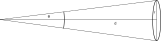
\includegraphics[width=0.8\columnwidth]{SmallAngles.pdf}
\includegraphics[width=0.4\columnwidth]{Eprofile_Lightson_Example.jpg}\includegraphics[width=0.4\columnwidth]{Eprofile_Grid_Example.jpg}
\caption{Eprofile example with grid. Left: reference, right: eprofile signal with grid.}
\end{figure}

Assume a point source that propagates and diverges over a distance $d$ until it is detected at the beam profile, now extending to a circle of radius $r$. If $d \gg r$, then the small angle approximation holds:

\begin{equation}
\tan \theta \approx \sin \theta \approx \theta, \quad \sin \theta = \frac{r}{d} \longrightarrow \theta \approx \frac{r}{d},
\end{equation}
where $\theta$ denotes the divergence, equivalent to the ratio of forwards to transverse momentum, $p_\parallel/p_\perp$.
\vspace{\baselineskip}

The pointing fluctuations of the beam can be estimated similarly if one suspects mainly an angular jitter. In reality the pointing will be related to a combination of translation and rotation, where a transverse displacement of the beam is typically of order $\sim \mu m$ and will then over the course of a drift be dominated by the angular displacement.

To obtain an absolute number for the divergence and pointing the screen has to be spatially calibrated. This includes characterising the relative angle of screen, camera and laser axis.
A regular grid of known dimensions, for instance printed on some paper, can be used as spatial reference to evaluate the relative angle of camera and screen. The angle of the screen relative to the beam has to be measured separately. 
One way to compensate both is to place the screen at 45 degrees to the beam and the camera looking at 45 degrees as well restoring the right dimensions.

\subsection{Magnetic Energy Spectrometer}

The energy of electrons in wakefield experiments can be determined in experiment using a spectrometer based on magnetic dispersion. The electrons are deflected using a dipole magnet and are detected on a scintillating Lanex screen.

In order to understand the fundamental relations this method is based on, the motion of a single electron in a homogeneous magnetic field is considered and analytically solved in the case of an electron passing through a region of a homogeneous magnetic field of finite extent, but without considering fringe fields or gradients. In reality, the magnetic fields are measured or simulated and particle tracked using numerical methods.
\vspace{\baselineskip}

Consider an external magnetic field restricted to a circle of radius $r_b$ embedded in an otherwise completely field-free region. The following derivation is based on Stuart Mangles' (Imperial College) PhD thesis \cite{ManglesThesis}.
\begin{align}
\mathbf{B} &= B \mathbf{e_z} \, &r \leq r_b,\nonumber \\
&= \mathbf{0} &r > r_b
\end{align}

The angular deflection of a particle in this case can be solved analytically using the Larmor radius and simple geometry.

\begin{figure}
\centering
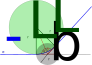
\includegraphics[height=0.3\columnwidth]{elecspec.png}\includegraphics[height=0.3\columnwidth]{Espec_shotexemp.jpg}
\includegraphics[width=0.75\columnwidth]{TrackingFigMangles2015.png}
\caption[Visualisation of an electron deflected in a homogeneous magnetic field and ]{Visualisation of an electron deflected in a homogeneous circular magnetic field (grey) with radius $r_b$. The larger green circle indicates the Larmor radius, determining the electron trajectory (blue) from the point of entry into the field (A) to its exit point (C) resulting in a total deflection $\theta$. Bottom: Example of particle tracking through a three-piece magnet for electrons of -X, 0 and +X MRAD pointing.}
\end{figure}

Drawing the circular field region for the magnetic field and the electron entering the field, one can then graphically indicate its Larmor radius, equivalent to its expected motion for the region with the constant B-field. The angles in this constellation are determined using the trigonometric relation that the angles in a triangle have to add up to $\pi$:
\begin{equation}
2 \alpha + \theta = \pi,
\end{equation}
where $\theta$ is the deflection angle and $\alpha$ the angle indicated in the graphic (see figure).

Relating this to the angles to substitute $\alpha$:
\begin{equation}
\tan \alpha = \frac{r_L}{r_b},
\end{equation}
and then expressing this into parameters we can measure in experiment we reach
\begin{align}
\tan \frac{\theta}{2} &= \frac{r_b}{r_L},\nonumber\\
&= \frac{e B r_b}{p_\perp}.
\end{align}

In a typical LWFA experiment $p_\perp$ will be dominated by the component in the laser propagation axis, i.e. if the propagation axis were z, $|\mathbf{p_\perp}| \approx p_z$. 
\vspace{\baselineskip}

\iffalse
\begin{figure}[h]
\centering
\includegraphics[width=0.75\columnwidth]{ExpSetup_GasJet_MagnetOnly.pdf}
\caption{Sketch of a typical spectrometer setup in a LWFA experiment (left). The relativistic electron (blue) beam enters the dipole magnet (grey) and is dispersed onto the lanex screen according to its energy. Higher energies are deflected less than lower energies. The image on the right is an example of a spectrum taken on an experiment. The high energies are on the bottom of the spectrum decrease with height upwards.}
\end{figure}
\fi

The correct assignment of the position on the screen to the correct electron energy is achieved by measuring the position of all components (lanex screen, magnet, TCC) and mapping the magnet field strength accurately, for instance using a Hall probe, and then running a particle tracking code with these details.
Each pixel has a certain error bar on its associated energy as the divergence of the electron beam (instrument function), an offset at source or shot-to-shot pointing fluctuations could lead to different positions at the same electron energy (pointing). The energy resolution is determined by the strength of the magnetic field, the drift length, the intrinsic spatial resolution of the scintillator (for Lanex $\sim 100\,\mathrm{\mu m}$ REF) and the spatial resolution of the imaging system. 
\vspace{\baselineskip}

A second Lanex screen or other spatial references (fiudicials) can help to identify and correct for pointing fluctuations or an overall pointing to achieve a more accurate determination of the energy, but could introduce additional scattering. See Kristjan Poder's PhD thesis \cite{PoderThesis} for more details on this or for instance \cite{Soloviev2011_TWOSCREEN}.

The width of the electron trace in the non-dispersion direction can be used to determine the divergence of the beam (in the non-dispersion axis) and cross-checked with the spectrum of the betatron radiation or a beam profile monitor.
\vspace{\baselineskip}

In addition to measuring the distances and the magnetic field, the imaging system for the scintillator screen has to be characterised.
This requires transforming the optical image (projective transform), spatially calibrate the image and translate from spatial to energy axis.
More details on the typical procedure can be found, for instance, in Jason Cole's or Kristjan Poder's PhD thesis \cite{ColeThesis, PoderThesis}

In all Chapters Lanex (standard and Biomax) are used in conjunction with Andor Neo cameras.

\iffalse
%\subsubsection{Multiple screens and deconvolution}

In a magnetic spectrometer electrons are being dispersed in one axis and the spectrum can be deduced from the fan of electrons and the position at a detector screen. Whereas the spatial extent in the non-dispersion direction tells us the divergence of the beam in that axis as it is approximately unperturbed, the divergence of the beam in the dispersion direction is convolved with the magnetic dispersion. At the same time an overall pointing of the beam could lead to an overestimate or underestimate of the actual energy. In order to be able to correct for these factors several points of reference are required. The source position has to be known along with two more measurements. This could be two screens or a spatial feature (fiudicial) and one screen.
A simple symmetry assumption mainly allows adding an error bar to the maximum energy within a reasonable limit.

Two screen tracking: forwards or backwards method.
Run tracking with a variety of angles for identical energies. Check what energy estimate each screen gives at a distinct feature. See if there are any deviations, try the next angle and find the least square fit.
The other approach is backtracking but this is more complicated.

If one has a fiudicial no explicit features in the beam are required as the fiudicial will become that feature. However, the positions have to be measured to a high precision to be able to distinguish sensible pointing shifts.

Either methods can be used to deconvolve the spectrum and iteratively find the real energy spectrum underlying the measured distribution. More screens can increase the accuracy but the scattering of the beam passing through lanex becomes quite evident and distinct features blur out when drifting further because of this.
\fi

\subsection{Absolute Charge Measurement}

Absolute charge measurements are challenging in an EMP rich environment as near intense laser-plasma interactions.

Commonly, Lanex or other scintillators imaged by optical CCD cameras are used to measure the electron spectrum and charge.
However, obtaining an absolute charge calibration requires a very detailed knowledge of the efficiencies of the scintillator material, imaging system, quantum efficiency of the detector chip and so on (REF REF). Typically, phosphorescent image plates (WHAT ARE THEY MADE OF) are used instead to achieve an absolute calibration (REF).

In the experiments described image plate was attached to the back of the electron spectrometer screen and left in the beam path for several shots. After removing the image plate again they are left to decay over a certain period before then being analysed using a scanner. The accumulated signature on the image plates was then overlapped with the corresponding scintillator images taken with the optical cameras to obtain a conversion factor of pixel counts to charge. The scattering and damping of the imaging plate has to be considered and its heightened sensitivity which might result in additional background noise on the imaging plate due to its large dynamic range.

The disadvantage of imaging plate technology is that it is not suitable for high repetition rate operation as it has to be replaced manually. In addition, any change of the imaging system requires a new calibration which could be intrusive and time-constraining depending on the spectrometer setup (vacuum or air?).
The evaluation of the diagnostic is also not instantaneous as it has to be left to decay and then scanned.
\vspace{\baselineskip}

Other technology being used are ICT, but they have to be shielded properly as electronics is vulnerable in EMP environment and are very expensive.


ADD A REFERENCE THAT DESCRIBES THE PROCEDURE IN MORE DETAIL, ON ABSOLUTE CALIBRATION.



\section{X-ray and Gamma-ray Diagnostics}

Wakefield acceleration has not only demonstrated to be a feasible tool to accelerate electrons to a GeV scale, but has also been shown to be a useful source of X-rays of remarkable brightness by the means of betatron radiation \cite{Rousse2004_BETATRON,Kneip2010_BETATRON}, as a tunable all-optical Compton-source \cite{TaPhuoc2012_ICS} and as bremsstrahlung source \cite{Glinec2005_Brems,Cipiccia2012_Brems}. In addition, using LWFA electron beams for FEL operations has become an active field of research itself (REF REF).

The following section addresses different diagnostics to characterise high-energy radiation produced using an LWFA source, laser-solid, laser-electron and electron-solid interactions.

\subsubsection{Motivation for variety of diagnostics}

In the following chapters various arrays of scintillator arrays (in this case caesium-iodide doped with thallium, CsI(Tl)) are employed to measure the spectrum of gamma radiation from various sources (bremsstrahlung, linear and non-linear inverse Compton scattering and hard betatron radiation).


In the soft and hard X-ray regime spectra can be deduced by comparing the transmission of the radiation through various materials with characteristic K-absorption edges (REF), Ross filter pairs (REF) or relying on crystal reflections matching the Bragg-condition (REF) or a combination of both.
For these conditions a good knowledge of the material properties and the positioning of the crystal and cameras is essential.
The energy-dependent transmission through the material is related to an interplay of different mechanisms (Compton scattering, Rayleigh scattering, photoelectric effect, pair production and so on). The sum of these cross sections can be combined and found in specific repositories (REF NIST).

At higher X-ray energies entering the gamma regime $\hbar \omega \rightarrow 1\,\mathrm{MeV}$ K-edges to effectively distinguish spectral bands become rarer and most materials become more transparent, as a consequence resolving a full spectrum becomes challenging. At the same time incoherent scattering becomes more dominant and pair production becomes possible, with increasing likelihood at higher energies (see cross section PLOT XX REF).
\begin{figure}
\centering
\includegraphics[width=0.5\columnwidth]{XsecCsI.png}\includegraphics[width=0.5\columnwidth]{XsecLi.png}
\caption{Mass attenuation of CsI (left) and Li (right).}
\end{figure}

At the few MeV level the spectrum of the generated electron-positron pairs scales directly with the energy of the gamma radiation interacting with the matter through Compton scattering (incoherent scattering) and pair production (REF). Measuring the spectrum of these particles, for instance with a magnetic spectrometer setup, and comparing the results with a simulation result can then be used to deduce a gamma spectrum \cite{Corvan2014_Gamma}. This works particularly well for low-Z materials as lithium (see PLOT) where the cross section for incoherent scattering dominates but also varies whilst the pair production cross section also strongly varies giving the diagnostic additional sensitivity.

\EliasComm{I checked and kevlar (so kapton will be very similar) has similar cross section for processes in the MeV range, so the vacuum window could act as converter.}

The spectrum of the pairs, however, becomes less sensitive to the energy of the gamma-radiation at higher (tens of MeV) energies (XSEC XX PIC REF). An alternative method to measure such a hard spectrum is tracking the energy deposition of radiation and secondary sources throughout an array of scintillator material until it decays, effectively measuring the length and shape of the cascade.
This method has the advantage of being variable and viable for the few MeV level and much harder radiation.

Simulations linked to this technique are outlined in this work and are then applied to experimental data in the following chapters to measure radiation from different materials in a range of hundreds of keV to hundred MeV (over three orders of magnitude).

A detector interacting with such high energetic gamma-radiation is now faced with energy deposition by the radiation itself and secondary particles and radiation. An extended detector can mitigate this effect by forcing pair production in an earlier part of the detector and performing an again well resolved measurement in a second part of the detector. The complex interplay of pair production and energy deposition from secondary sources requires numerical solutions calculating the cross-sections for various processes dynamically throughout the interaction with the detector. The extended detector acts as an imperfect calorimeter with some energy resolution. This is where GEANT4 \cite{GEANT4} or other Monte Carlo based simulation codes come into play (e.g. \cite{MCNP}).

\subsection{Pinhole Camera}

A pinhole camera is a relatively simple diagnostic that allows measuring the source size and estimate the flux of an X-ray source.

CCD Chip, pinhole of right material on tube to shield noise, source. Relative distances determine the magnification (geometric magnification).

geometric magnification M: distance camera to source
\begin{equation}
M = \frac{d_{cam-pin}}{d_{source-pin}}
\end{equation}


Used on the experiment described in Chapter XX.

Double pinhole, one with 5 um aluminium and one with 6 um PET filtering. The pinhole itself is made of 25 um Ta.
X-ray cameras used are DX420-BR-DD Andor in-vacuum cameras with XX times XX chips each XX times XX microns. These are sensitive to X-rays, see QE curves XX REF. Quite often with beryllium window or filtering in front of the chip.

Alignment can be done by adding a spike on the front, point it at the interaction point and then carefully removing it at the end.

By comparing the transmission of the two spots (using a double pinhole) gives an estimate how much energy is in one band and another, especially if the K-edges are chosen correctly.
\begin{figure}
\centering
\includegraphics[width=0.9\columnwidth]{PinholeCamera.png}
\includegraphics[width=0.9\columnwidth]{20180326r001s002_PinholeCam.jpg}
\caption[Example of pinhole camera image.]{Top: Sketch of a pinhole camera. Bottom: Example of a double pinhole camera image taken on a recent experimental campaign. The pinholes were filtered differently, such that the pinholes measure the flux in different spectral intervals.}
\end{figure}

\EliasComm{Refer to BK's thesis \cite{KettleThesis}.}


\subsection{Crystal Spectrometer}

Bragg condition and crystal, CCD camera.
Applicable in any range accessible using lattice constants. Energy range depends on detector size, distance and lattice properties.

Bent crystals can be used for focusing and larger spectral range.
HAPG HOPG with mosaicity to increase reflectivity.

Bragg's law

\begin{equation}
n \lambda = 2 d \sin \theta
\end{equation}

Energy spread/error on the camera based on initial divergence.

Efficiency needs to include reflectivity of crystal, filtering, quantum efficiency and so on. Thermal noise.

Used in experiment described in Chapter \ref{Chap:BW}.
\begin{figure}
\centering
\includegraphics[width=0.5\columnwidth]{CrystalSpecCamera.png}
\includegraphics[width=0.9\columnwidth]{CrystalSpec.pdf}
\caption[Sketch of a crystal spectrometer setup.]{Top: Sketch of a crystal spectrometer setup. X-rays are dispersed onto a CCD chip. Bottom: Example of a spectrum measured in a crystal spectrometer setup. The X-rays are dispersed spectrally in the x-axis with distinct emission lines. The central part is filtered with aluminium, resulting in a sharp cut-off due to the K-edge, which can be used as calibration.}
\end{figure}

\EliasComm{Refer to BK's thesis \cite{KettleThesis}}

Andor DX420 in-vacuum cameras (since we are looking at very fine resolution and low energies).

Pixel size for the cameras and typical filtering.

REF BK thesis, sketch also based on one of his sketches.

Applications for XANES measurements due to good resolution \cite{Kettle2019_XANES}.

The K-edge of a filter can be used to get an on-shot energy reference to calibrate the image. Two different materials would make this even clearer.
The sharpness of the edge could be an indicator of energy spread/divergence impact. Few eV resolution.

See FIGURE REF for example of a spectrum taken on an experiment. Spectral lines and K-edge from aluminium filter.

In this range the accurate knowledge of the filtering (micron thickness) is crucial as this is the few keV range.

Have to use in-vacuum as going through a window would result in cut-out of the relevant signal.

\subsection{Filter Packs}

Typically used for X-ray measurements on LWFA experiments (betatron radiation) are filter packs or arrays of materials of varying K-edge over the range of X-ray energies expected. By comparison of the transmission through the materials and assuming a spectral shape, the spectrum can be estimated. The profile of the radiation is also measured but has to be corrected for when comparing the transmissions.

Direct (CCD) or indirect detection (with scintillator) Andor iKon.


\begin{figure}[h]
\centering
\includegraphics[width=0.9\columnwidth]{filter_pack_sketch.pdf}
\caption{Sketch of a typical betatron setup.}
\end{figure}


\begin{figure}
\centering
\includegraphics[width=0.3\columnwidth]{FilterPack.png}\includegraphics[width=0.3\columnwidth]{FilterPackX.png}
%\includegraphics[width=0.3\columnwidth]{QE_BR_DD.png}\includegraphics[width=0.3\columnwidth]{DeltaEcrit.png}
\caption{Images of filter packs.}
\end{figure}

When X-rays increase in energy the quantum efficiency of the CCD chip decreases, so energies beyond 100 keV are not measured.

More details on the extraction procedure can be found in Jonathan Wood's PhD thesis \cite{WoodThesis}.

Was not used on the experiments described in this work but other relevant experiments.
To motivate why other indirect detection methods are required and this method becomes less sensitive at higher energies.

If we assume only absorption following Beer's law, the signal through a filter on the camera including quantum efficiencies (QE) etc. (taken from Jonathan Wood's PhD thesis \cite{WoodThesis})

\begin{equation}
Y_i = A \int^{E_{max}}_{E_{min}} E \,S(E) \,Q(E) \,T_i(E) \,\mathrm{d}E
\end{equation}

Then minimise (least square) the transmissions for a spectrum S(E).

\subsection{Gamma-ray Scintillator Profile}

Once the energies reach the gamma-ray regime (> 1 MeV), even using an indirect-detection camera on axis becomes infeasible as photons will decay into secondary particles and radiation that will shower the camera and reduce its lifetime.

Relying on indirect detection with an off-axis camera or detector then becomes necessary. 
In experiment this has been an array of scintillator material normal to the beam axis and imaged by a camera.

This enables measuring the shape of the profile is interesting as it allows deduction of the source (SEE REF). In this context it gives insight into the properties of the electrons (their divergence, propagation and so on). 
The profile is also an indicator the the intensity of the interaction in non-linear ICS and carries the imprint of the interacting electron beam within it.
It is hence a useful diagnostic to not only confirm an interaction took place but also to characterise the conditions at the interaction.

\EliasComm{Reference REF UMSTADTER AO? TOM BLACKBURN IF PUBLISHED.}

\subsubsection{Experimental Implementation}

In these experiments caesium-iodide doped with thallium is used frequently due to its high light yield. LANEX has typically a better spatial resolution due to its fine grain size ($\sim 100\,\mathrm{\mu m}$) but the energy deposition in the thin screens, especially at gamma-ray energies, is not sufficient to produce a lot of signal. Long CsI crystals give a pixelated response. LYSO also comes at a decent resolution but the light yield is lower. It is a fast scintillator but at lower repetition rates as at Gemini, this is not necessary and the noise levels can not be gated away as it is too close.

\begin{figure}
\centering
\includegraphics[height=0.3\columnwidth]{JenaProfile.jpg}\includegraphics[height=.3\columnwidth]{ScreenshotGEANT_JenaStack.png}\includegraphics[height=0.3\columnwidth]{20190208r015s036_GammaProfile_crop.jpg}
\caption[Scintillator profile screen, photograph, GEANT representation and measured gamma signal.]{Example of a scintillator stack used as profile screen in experiment. Photograph of the scintillator screen (left) along its GEANT representation (middle) and gamma signal measured with the stack in experiment (right).}
\end{figure}

Different profile screens were used in the experiments. The details can be found in Table XX NUMBER REF.

The scintillators emit around 546 nm (XX NUMBER) of radiation which is ideal for CCD chips. Andor iXon cameras (sensitive chips) are used to image the scintillators close to normal or using a mirror. A bandpass filter can be used to reduce the noise.


\begin{table}[h]
\centering
\begin{tabular}{l|l|l|l|r|r}
Name & Chapter &Crystals & Crystal Dimension & Front Plate & Divider\\ \hline \hline
QUB & \ref{Chap:BW}, BW & $20 \times 20$ & $2 \times 2 \times 20$ mm & Al 10 mm & Al 0.1 mm\\
Jena & \ref{Chap:linICS}, linICS & $45 \times 45$ & $1 \times 1 \times 10$ mm & TiO2 0.5 mm & TiO2 0.2 mm\\
DESY & \ref{Chap:linICS}, linICS & $30 \times 30$ & $1.5 \times 1.5 \times 10$ mm & Epoxy 0.5 mm & Epoxy 0.2 mm\\
RAL & \ref{Chap:RR15}, RR & $47 \times 33$ & $5 \times 5 \times 50$ mm & None & Al 1 mm
\end{tabular}
\caption[Overview of CsI profile screens used in experiments.]{Overview of caesium-iodide crystal stacks used in experiments as profile screens.}
\end{table}

The photons go through the entire thickness of 10 mm CsI, so background subtraction from random noise was not a large concern. The signal is strong, also due to the high light yield of CsI at cost of spatial resolution (1mm crystals). The crystal outlines themselves and the overall array act as spatial reference as their symmetry is well known. A close to normal orientation is preferable to discourage mixing and again a normal imaging is ideal as well, resulting in very little post-processing being required.



\subsubsection{GEANT simulations showing energy deposition}

\EliasComm{Add a figure on energy deposition using GEANT REF for MeV range and on the other hand absorption using Henke.}
RESULT: The energy deposited in an energy range (GIVE GEANT SIM FOR 10-XX MEV) is proportional to the energy of the radiation.

\EliasComm{Add comment on GEANT code in general, REF GEANT, mention Jason's and Kris' input.}

When planning to use such a detector as measurement of the total energy of the radiation one has to keep in mind that this is not a calorimeter in the gamma regime as radiation is bound to be transmitted through the stack. However, it is expected that the energy deposited per photon will vary and of course the number of photons will leave their trace on this detector.

The response is simulated using GEANT:
The detector in the simulation:
the detector assembled in the simulation is based on a CsI stack used in some experiments and provided by the Helmholtz Institut in Jena.
It consists of 45 x 45 CsI(Tl) crystals of face dimension 1 mm x 1 mm and a thickness of 10 mm. The crystals are spaced by a 0.2 mm layer of TiO2 and the front side has another layer of TiO2 of 0.5 mm which holds the entire stack together.

The stack was defined as such in the simulation and it can be seen in Figure ADD HERE.


The front side of the detector is XX m away from the source of the radiation, similarly to experiment conditions, hence being in general able to cover plus minus NUMBER divergence from a point source if centred along the same axis.

Now individual photons with ranging energy from 10 keV to 500 MeV are launched from the source point and the energy deposited in the crystals is being recorded. Each energy step is simulated 10.000 to 100.000 times and then averaged to obtain an average energy deposited per photon of this energy.

The results from these simulation can be seen in figure ADD HERE. Photon energies up to ENERGY are almost completely absorbed, backscattered and rarely transmitted. At around 200 keV suddenly a large amount of radiation is being absorbed. This indicates a material characteristic absorption edge.
This means that whilst for the majority of the energy ranges the CsI profile will give a good indication as energy times flux is monotonic increasing and somewhat linear for the two regimes of interest. In the regime of hundreds of keV we have to consider that a lot of energy will be absorbed in the front layer and we have to check how this behaves further downstream in the next detector.

\begin{figure}
\centering
\includegraphics[width=.5\columnwidth]{Edep_JenaStack.pdf}\includegraphics[width=.5\columnwidth]{Edep_JenaStack_rel.pdf}
\caption{Simulation results: energy deposited per photon in a profile stack. Replace this by 10's MeV plot as GEANT is not performing too well at low keV levels and the 250 keV peak might be a fluke.}
\end{figure}

If we look at this in terms of relative energy deposited per photon, so in other words energy deposited over energy of the photon, this does not look like a sharp edge but merely a steady decrease in energy deposited relative to the total photon energy. Scattering cross sections typically decrease with increase in energy and this goes along the same lines.


\subsubsection{Absolute Calibration}

The smaller profile stacks can also be calibrated by using a radioactive source since the stack mainly consists of crystals.
A Na or Cs source can be used at the standard measurement conditions. The energy emission is well known. If one assumes that all energy is absorbed by the detector the light yield is related to energy deposited. The disadvantage to real calorimeters is that due to a non-zero transmission through the material and due to the spacers not all energy deposited is deposited within crystals and converted into signal.



\subsection{Gamma-ray Converter Spectrometer}

At gamma-ray energies above $2m_e c^2 \approx 1\,\mathrm{MeV}$ one photon can generate a pair of electron-positron pairs when scattering from matter using the electric field of the nucleus or the valence electrons as interaction partners. The maximum energy of the generated electrons and positrons are determined by the energy of the gamma photon, the overall spectrum is close to exponential (SEE THEORY INSERT REF, BETHE HEITLER). Based on this principle one method to measure the gamma spectrum is using a sheet of high-Z material to convert the gamma rays into matter and then measure the spectrum of these particles in a magnetic spectrometer (REF).
\EliasComm{Need to rework this part since it is not just pair production but also Compton scattering.}
In the range of few to maybe 30 MeV the cross section rises rapidly (SEE FIGURE XX NUMBER) compensating for the fewer pairs at higher energies and making this a feasible spectrometer to resolve the full spectrum in this range \cite{Corvan2014_Gamma}. At higher energies the cross-section flattens which means that the contribution to the total production of pair equalises over all energies but due to the exponential spectrum of the pairs produced very few pairs at the maximum photon energies are produced.
The Compton spectrometer becomes a pair spectrometer and the signal-to-noise ratio and sensitivities become more important, meaning more space is required to resolve those energies since the higher energy pairs now require stronger magnets, more drift and need to clear away from the noisy axis.
 
\begin{figure}
\centering
\includegraphics[width=0.5\columnwidth]{CorvanSpectrometer.png}
\caption[Sketch of a Compton spectrometer design.]{Sketch of a Compton spectrometer design: gamma rays enter the setup from the left side and enter a block of lithium, releasing electrons through Compton scattering and depending on the energy also electron-positron pairs. A magnetic field disperses electron and positrons onto detector screens. Reprinted from \cite{Corvan2014_Gamma}, with the permission of AIP Publishing.}
\end{figure}

